\documentclass[a4paper,man,natbib,floatsintext,donotrepeattitle]{apa6}

\usepackage[english]{babel}
\usepackage[utf8x]{inputenc}
\usepackage{amsmath}
\usepackage{graphicx}
\usepackage[colorinlistoftodos]{todonotes}
\usepackage{xcolor}
\usepackage[draft,inline,nomargin,index]{fixme}
\usepackage{hyperref}
\usepackage{verbatim}
\usepackage{nameref}
\usepackage{booktabs}
\usepackage{lineno}
\linenumbers

\fxsetup{theme=color,mode=multiuser}
\FXRegisterAuthor{ab}{sab}{\color{blue}Amelie} % abnote{} with text inside to edit
\FXRegisterAuthor{bb}{sbb}{\color{purple}Brice} % bbnote{} with text inside to edit
\FXRegisterAuthor{ln}{sln}{\color{violet}Lad} % lnnote{} with text inside to edit

%\title{Blinding as a Necessary Precaution Against Experimenter Biases During Sequential Bayes Factor: A commentary on \cite{schonbrodt_sequential_2017}}

%\title{On the importance of blinding during sequential testing procedures: A commentary on \cite{schonbrodt_sequential_2017}}

\title{"Efficient" yes, but only if you blind yourself: A commentary on \cite{schonbrodt_sequential_2017}}

\shorttitle{Blind Bayes Factor}
\threeauthors{Amélie G. Bret}{Brice Beffara}{Ladislas Nalborczyk}
\threeaffiliations{Univ. Grenoble Alpes, CNRS, LPNC UMR 5105, F-38000, Grenoble \\Psychological Science Research Institute, Catholic University of Louvain, Belgium}{The Walden III Slowpen Science Laboratory, France}{Univ. Grenoble Alpes, CNRS, LPNC UMR 5105, F-38000, Grenoble \\ Department of Experimental Clinical and Health Psychology, Ghent University}

\abstract{In this commentary we discuss potential issues associated with the Sequential Bayes Factor procedure as introduced by \cite{schonbrodt_sequential_2017}. We argue that particular precautions should be undertaken to ensure objectivity during sequential testing procedures (both Bayesian and frequentist). More precisely, we highlight the need for triple-blinding during such procedures, and provide recommendations on how to implement this without additional costs.}

\keywords{sequential testing, triple-blind, research methods}

% re-enabling section numbering (disabled by the apa6.csl)
% \setcounter{secnumdepth}{3}

\begin{document}

% defining a new command for counting words
\newcommand{\quickwordcount}{%
  \immediate\write18{texcount -1 -sum -merge \jobname.tex > \jobname-words.sum }%
  \input{\jobname-words.sum}words%
}

\maketitle

Wordcount: This document contains \textbf{\quickwordcount}.

\newpage

\tableofcontents % provisoire, juste pour se repérer entre nous
\newpage

% Notes
% répartition des tâches: Lad intro, Brice experimenter biases, Amélie blinding, et tout le monde section 3 et conclusion

%%%%%%%%%%%%%%%%%%%%%%%%%%%%%%%%%%%%%%%%
% début du comment
%%%%%%%%%%%%%%%%%%%%%%%%%%%%%

\newpage

\section{Introduction}

\subsection{Context}

\cite{edwards_ward_bayesian_1963} state, "the rules governing when data collection stops are irrelevant to data interpretation. It is entirely appropriate to collect data until a point has been proven or disproven, or until the data collector runs out of time, money, or patience". However, as noted by \cite{schonbrodt_sequential_2017}, "this practice of unplanned multiple testing is not allowed in the classical NHST paradigm, because it increases Type I error rates". They add: "\textit{Of course, one can calculate statistics during data collection, but the results of these tests must not have any influence on optionally stopping data collection}."

In this short commentary, we will argue that such interim analysis (including visual inspections of the data) might have an influence on future data collection and optional stopping through overlooked experimenter biases, thus biasing the expected results of sequential testing procedures (both Bayesian and frequentist). Because we acknowledge and appreciate the huge contribution brought by the seminal work of \cite{schonbrodt_sequential_2017}, in the second part of this commentary we will highlight quick fixes / methodological precautions that will ensure the efficiency of the SBF procedure.

\subsection{The SBF design}

In their paper, \cite{schonbrodt_sequential_2017} present an alternative to the much used NHST with a priori power analysis (NHST-PA). They introduce the \textit{Sequential Bayes Factor} (SBF) procedure that allows to collect data iteratively, until a predefined threshold is reached, while not suffering from the pitfalls associated with similar procedures used in the NHST framework. Testing mean differences between two independent groups, they show that the SBF design typically needs 50\% to 70\% smaller samples to reach a conclusion about the presence of an effect, as compared with optimal NHST-PA (where \textit{optimal} stands for an idealized situation in which the a priori targeted effect would be exactly equal to the \textit{true} effect size), while having similar long-term error rates.

% With this in mind, it is striking to see that though double blinding procedures have became a gold standard in many psychological fields, much less attention has been dedicated to triple blinding (i.e., procedures ensuring that the person who analyses the data is blinded to hypotheses).

However, while it seems an attractive perspective and while we generally agree with most of their recommendations, we wanted to raise some concerns about precautions that need to be undertaken in order to preserve the long-terms rates of wrong inferences they provide. One major concern is that the person who runs the experiment and the person who analyses the data are usually the same person. As noted by \cite{wicherts_degrees_2016}, in the psychological field, "the analyses are typically conducted by a person who is not only aware of the hypotheses, but also benefits directly from corroborating them". Thus, failures of blinding procedures are listed among the 34 researchers degrees of freedom identified by \cite{wicherts_degrees_2016}. In the current commentary we want to highlight the particular dramatic consequences of blinding failures in the context of sequential testing.

\section{SBF procedure: A social situation}

...a psychological experiment is a social situation / process...\cite{rosenthal_social_1963,rosenthal_experimenter_1964}...échantillonnage biaisé: on atteindra plus vite / plus lentement le seuil pré-défini...see Figure \ref{fig:diag1}...created with https://www.draw.io/ ...

\begin{figure}[H]
  \caption{Overview of the SBF procedure and illustration of potential biases when the experimenter and the data analyst are the same person.}
  \centering
  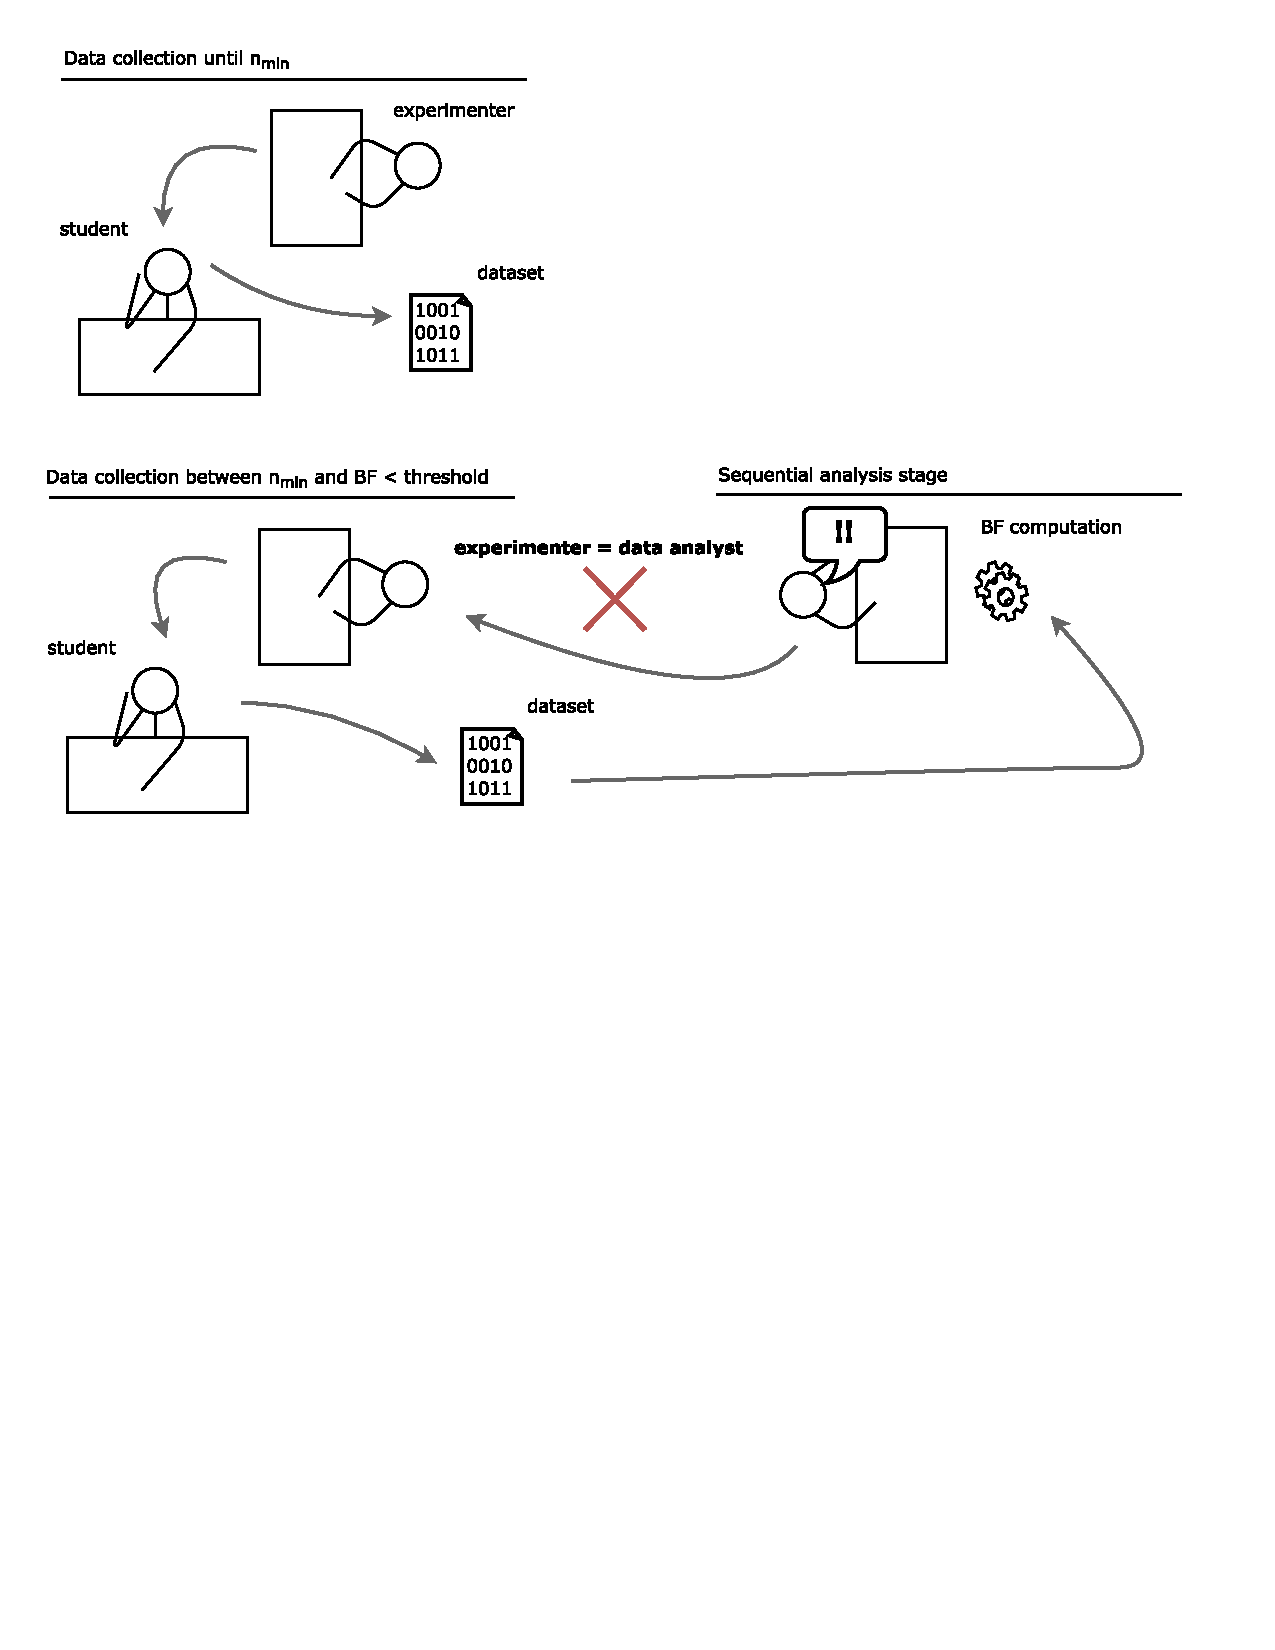
\includegraphics[width=0.8\textwidth]{figures/bias_diag.pdf}
  \label{fig:diag1}
\end{figure}

...Sequential-Experimenter-Analyst-Bias (SEAB)...direct consequence of the SEAB is that it introduces a time dependency between participants...this kind of auto-correlated data would invalidate the use of the models compared by...in their original paper...

\section{What does look like the SEAB ?}

The SEAB can wear a multitude of forms as it is a function of the researcher \textit{a-priori} expectancies and of the \textit{true} effect size. Moreover, we focus here on the simplest case in which the expectancies of the researcher remain constant throughout the sequential testing procedure. Although maybe non realistic, this setting serves illustrative purposes in the next section.

\subsection{Predictions}

Below we describe four situations that are faced everyday... \lnnote{created with https://www.tablesgenerator.com...}

\begin{table}[H]
\centering
\caption{Four usual situations in the experimental setting}
\label{tab:pred}
\resizebox{\textwidth}{!}{%
\begin{tabular}{@{}ccc@{}}
\toprule
 & \begin{tabular}[c]{@{}c@{}}There is no difference in the population\\ (H0, d = 0)\end{tabular} & \begin{tabular}[c]{@{}c@{}}There is a difference in the population\\ (H1, e.g., d = 0.6)\end{tabular} \\ \midrule
Researcher 1, believes in H0 & Panel A (congruent) & Panel B (incongruent) \\
Researcher 2, believes in H1 & Panel C (incongruent) & Panel D (congruent) \\ \bottomrule
\end{tabular}%
}
\end{table}

...Figure \ref{fig:pred} illustrates our predictions for the 4 scenarios presented in Table \ref{tab:pred}...created with https://www.draw.io ...

\begin{figure}[H]
  \caption{Predicted consequences of the SEAB on the results of a SBF procedure, for a given Cohen's d of 0.6 (hereafter, "H1") or of 0 (hereafter "H0"), according to the \emph{a priori} researcher beliefs.}
  \centering
  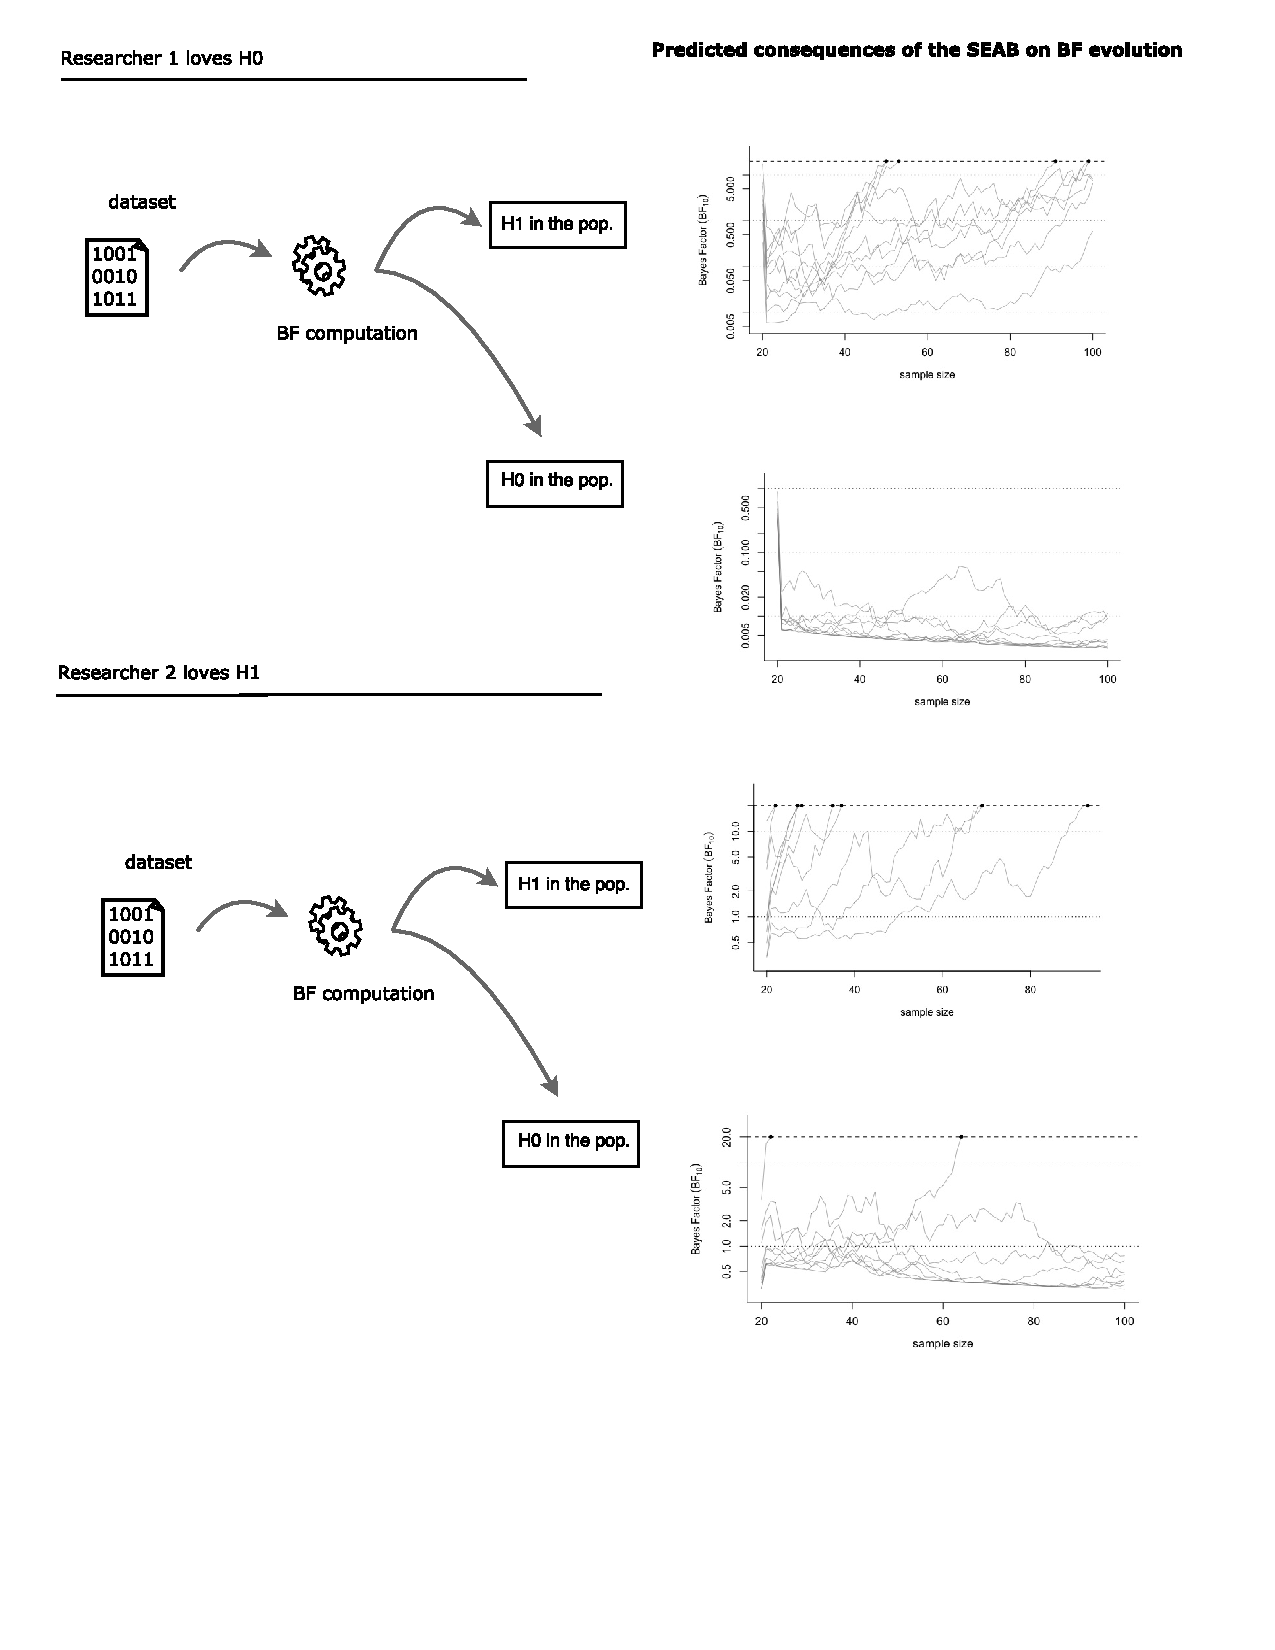
\includegraphics[width=0.8\textwidth]{figures/BFF_predictions.pdf}
  \label{fig:pred}
\end{figure}

\lnnote{peut-être ajouter un plot de l'évolution "normale" du BF pour la même taille d'effet ? et inverser le graphique pour faciliter la comparaison chercheur H0 vs/ chercheur H1}

\subsection{Experimental demonstration}

...proposer ici un protocole expérimental qui permettrait de mettre en évidence le SEAB... ou pas ?

\section{Solutions ? Blind yourself.}

...blinding (double or triple)...

\subsection{Solution 1: one analyst, one experimenter}

...blah blah...

\subsection{Solution 2: one analyst-experimenter, "software-blinded"}

...this solution is relatively costless. To demonstrate this, we added a very short append to the \texttt{seqBF} function, written by Félix Schönbrodt \& Richard Morey (available \href{https://raw.githubusercontent.com/richarddmorey/BayesFactorExtras/master/BayesFactorExtras/R/seqBF.R}{here}), so that the user can now simply set the \texttt{blind} argument to \texttt{TRUE} and thus be completely blind to the results of the sequential BF computations. The only output is a sentence that either indicates to "continue" or to "stop" the recruitment, considering an a-priori defined threshold (see \nameref{sec:supp} for code details).

\section{Conclusions}

...exemple de manip utilisant le SBF: \cite{martin_perceiving_2016}...

\section{Supplementary materials}\label{sec:supp}

Reproducible code and figures can be found on Github: \url{https://github.com/lnalborczyk/Blind_BF}.

\lnnote{le repo est privé pour le moment donc on ne peut pas y accéder avec ce lien, mais la fonction est dispo sur le repo Overleaf.}

\section{Acknowledgements}

...many thanks to my mom...en plus de ma maman, peut-être faire relire ce commentary par des adultes avant de le soummettre ?...

\bibliography{BBF}

\end{document}
